% ---
% Capitulo de revisão de literatura
% ---

\chapter{Referencial Teórico}\label{referencial_teorico}

\subsection{DevOps}
O conceito de DevOps, acrônimo de \textit{Development and Operations},  pode ser entendido como o nivelamento entre as equipes de desenvolvimento e operações no que tange suas interações, mantendo funções específicas, porém alinhando suas demandas referentes às responsabilidades e processos, visando a disponibilização de um produto ou funcionalidade de forma rápida e confiável.\cite{gartnerglossario}

As implementações nesse tipo de ambiente fazem uso de ferramentas de automação com o intuito de dinamizar cada vez mais a infraestrutura e torná-la mais programável, de forma que reflita na melhoria contínua da comunicação e integração entre desenvolvedores e administradores de infraestrutura, transformando o cenário tradicional de isolamento entre essas duas equipes em um ambiente participativo e colaborativo.\cite{costa}

O objetivo do DevOps é gerar em toda a equipe envolvida na produção de um software, uma cultura que vise o aumento do fluxo de trabalho (maior frequência de deploys) e em paralelo a isso, dar mais robustez no desenvolvimento da aplicação. Esse conceito representa muito mais do que simplesmente o uso de ferramentas de automação, é importante observarmos que trata-se de uma quebra de paradigmas e uma mudança na cultura no negócio com uma nova forma de produção.\cite{sato2014devops}

A agilidade no processo de deploys citado anteriormente, aluz à uma necessidade de amparo para que essa entrega rápida de fato aconteça, e mais do que isso, a demanda por parte dos clientes ou usuários de determinada aplicação, requer cada vez mais velocidade no uso de certa funcionalidade. Analogamente à revolução industrial do século XX, a mudança na forma de produção de produtos naturalmente está sendo absorvida pela tecnologia, assim, a concepção desse produto deve acompanhar a demanda externa. A adaptabilidade e mudança da arquitetura funcional no desenvolvimento de serviços tecnológicos são necessidades relevantes, a cultura DevOps é uma mudança importante nesse ponto, e a definição de um ciclo contínuo do processo, como demonstra a Figura \ref{fig:figura1}.\cite{ibmdevops}

\begin{figure}[htb] %Figura: Ciclo de vida DevOps
	\centering
	\includegraphics[width=1\linewidth]{figura1}
	\caption{Ciclo DevOps}
	Fonte: Amazon Web Services, Inc., 2018
	\label{fig:figura1}
\end{figure}

Segundo uma pesquisa realizada pelo Gartner Group sobre DevOps, em 2015, somente 29\% das organizações pesquisadas tem esse modelo atuante em produção. É evidenciado ainda que apenas 42\% desses, tem a atuação do DevOps em aplicações móveis. De acordo com o mesmo grupo o DevOps evoluiria de uma estratégia de nicho para uma estratégia comum sendo empregada por 25\% das organizações do Global 2000\footnote{Forbes Global 2000 é uma classificação anual das 2.000 empresas públicas do mundo pela revista Forbes. O ranking é baseado em quatro critérios: vendas, lucro, ativos e valor de mercado. A lista é publicada desde 2003. Fonte: Forbes}.\cite{gartnerglobal}

O uso da cultura DevOps deve ser absorvida na necessidade de versionamento contínuo de determinada aplicação, ou seja, a frequente execução de deploys. Nisso, é importante observarmos que a rápida proliferação de software requer atualizações operando na mesma medida ágil e demandada pela competitividade de mercado, visto que a velocidade no atendimento da expectativa dos clientes diferencia a empresa em relação às demais atuantes no mercado.

A principal vantagem no uso de DevOps é a melhora evidente nos processos e automatização das tarefas, otimizando o tempo e reduzindo os ciclos de desenvolvimento. Por se tratar de uma interação entre as equipes de desenvolvedores e operacionais, dizemos que é um sistema bimodal de trabalho.\cite{sato2014devops}

O monitoramento de métricas e registro de logs é um aspecto relevante. Leva-se em conta que os serviços devem estar disponíveis 24 horas por dias e durante os 7 dias da semana, acarretando em uma massiva análise de dados e logs gerados pelo sistema, portanto, a rotina na observância desses elementos deve ser constante. É possível, inclusive, a criação de alertas que apontem situações e permitam a gerência proativa dos serviços\footnote{Atividades desenvolvidas com o objetivo de produzir, executar ou disponibilizar uma ferramenta que visem atender a necessidade do usuário}.

Outro benefício fundamental do DevOps é o aumento na comunicação e colaboração que envolve todos os personagens da empresa. É importantíssimo a definição de normas que permitam um maior compartilhamento de informações, ou que permita a proliferação da comunicação, seja qual for o método ou tecnologia, desde que agregue valor. Além disso, a diminuição de ruídos na comunicação e conflitos entre as equipes melhora o ambiente e tende a produzir efeitos positivos ao fim do processo.\cite{gaea}

Pode-se ainda elencar ganhos em maior estabilidade e melhor desempenho, e tão importante quanto, a redução considerável de custos de trabalho, visto que a diminuição de tempo de produção e menor esforço afeta diretamente o custo financeiro estimado em um projeto.


\section{Infraestrutura como Código}
Falar em infraestrutura com código é exatamente absorver o entendimento do tratar a estrutura de TI como um software, programável. Com isso é possível o uso de práticas que envolvam o controle por versionamento, testes automatizados, entrega contínua, entre diversos outros recursos por meio de scripts específicos.

O uso de práticas anteriores com métodos de gerenciamento de infraestutura foram válidos e deram uma base poderosa para a concepção de novas tecnologias. Atualmente, há  uma constante demanda de softwares cada vez mais dinâmicos e um alto índice de \textit{deploys}, inclusive simultâneos, levando à necessidade de concepção de uma infraestrutura que acompanhe o ritmo de complexidade desses novos sistemas.\cite{humble2014entrega}

Segundo a Hewlett Packard\footnote{Disponível em: https://www.hpe.com/br/pt}, em seu site oficial, a infraestrutura como código elimina a necessidade de criar diversos ambientes de produção de forma manual, isolada e separadamente, e/ou atuailzações de hardware e sofware. Toda essa dinâmica pode ser feita através de scripts contidos no mesmo conjunto de códigos, trazendo velocidade, economia e otimização de tempo. Nesse contexto, a infraestrutura como código traça uma linha tênue entre o código que executa a aplicação e o código que configura um ambiente, tornando um ambiente característico do DevOps.


\section{Ferramentas para Provimento de Serviços}
Apesar do conceito DevOps ser recente, a gama de ferramentas que contribuem para implantação dessa cultura já se mostram bastante diversificadas. Dentre as mais populares, destacam-se nesta seção um conjunto de ferramentas para provimento desses serviços.

\subsection{Atlas}
É uma ferramenta disponibilizada pela Hashicorp, que tem a função de unificar projetos \textit{open source} para o manejo de aplicações finalizadas no desenvolvimento para a produção em qualquer que seja a infraestrutura.
As etapas do Atlas seguem cinco passos, como demonstra a Figura \ref{fig:etatasAtlas}, isso independe da tecnologia utilizada, sejam máquinas virtuais ou contêineres, as etapas se mantêm as mesmas. \cite{hashimoto}

\begin{figure}[htb]

	\centering
	\includegraphics[width=0.8\linewidth]{etatasAtlas}
	\caption{Etapas do Atlas}
	Fonte: Hashicorp\footnotemark
	\label{fig:etatasAtlas}


\end{figure}
	\footnotetext{Disponível em: https://www.hashicorp.com/blog/atlas-announcement}




O Atlas não é um software de caixa preta, ou seja, é possível acesso a serviços que contribuem para tanto, como Vagrant\footnote{Disponível em: https://www.vagrantup.com/} (gerencia ambientes de desenvolvimento), Packer\footnote{Disponível em: https://www.packer.io} (construção de artefatos), Terraform\footnote{Disponível em: https://www.terraform.io/} (implantação de Infraestrutura) e Consul\footnote{Disponível em: https://www.consul.io/} (monitora os serviços em tempo real).

\subsection{Chef}

É um framework destinado à automatização para sistemas e infraestrutura em nuvem. O Chef\footnote{Disponível em https://www.chef.io} constrói, entrega e administra fazendo uso de scripts replicáveis.

O Chef tira a carga dos administradores de sistemas que focam no gerenciamento projetado para servidores autônomos, ele permite executar centenas de instâncias de servidor em um tempo imensamente menor se comparado ao uso comum em deploys. Para gerenciar esse tipo de configuração, o Chef, transforma a infraestrutura em código, deixando o processo mais flexível, legível pelos analistas e testável, possibilitando assim a gerência de recursos tanto localmente quanto na nuvem.\cite{lecheta2014aws}

Em sua topologia o Chef tem três principais componentes: o Servidor Chef, as Estações e o Nós. O maior atrativo dessa ferramenta é o uso de "cookbooks" ou receitas, são ditas configurações plugáveis, que envolvem todas as instalações e parâmetros necessários para atender determinada aplicação no servidor ou máquina. Assim como as receitas convencionais definem uma estrutura sequencial que deve ser seguida a fim de tornar o produto final reflexo de uma ideia original, o Chef mantém um conceito semelhante a isso, onde define-se um estado desejado do sistema, desenvolvendo um código de configuração, então processa-se esse código, une ao processo os dados do nó em questão e garante que o estado concebido seja correspondente ao estado do sistema. \cite{garzotto2006chef}

O Chef pode ser executado em várias plataformas, como Windows, distribuições Linux, FreeBSD, Solaris, AIX, Cisco IO e Nexus. E ainda suporta plataformas em nuvem,como Amazon Web Services (AWS), Google Cloud Platform, OpenStack, IBM Bluemix, HPE Cloud, Microsoft Azure e VMware vRealize.

\subsection{Docker}

O Docker\footnote{Disponível em https://www.docker.com/} é uma plataforma de automação que implanta as aplicações em espaços isolados chamados de \textit{contêineres}, possibilitando executar as aplicações de forma mais ágil. O objetvo é criar múltiplos ambientes dentro de um mesmo servidor, acessíveis externamente.

Essa ferramenta constrói a arquitetura do software de modo a tornar o armazenamento ainda mais robusto. A essência no Docker é acomodar os serviços ou aplicações em contêineres atômicos ou descartáveis. Em todo o processo de desenvolvimento, um contêiner pode ser excluído e ser restaurado se assim surgir a necessidade, isso torna a dinâmica de entrega e testes extremamente flexível.\cite{mattiaskane}

O Docker é uma plataforma \textit{Open Source}, que não pode ser confundido com um ambiente tradicional de virtualização. No Docker fazemos uso de recurso isolados que utilizam bibliotecas do kernel em comum, isso porque é presente nessa ferramenta o Linux Containers (LXC), a Figura \ref{fig:dockerXvm} apresenta isso.

\begin{figure} [htb]
	\centering
	
	\includegraphics[width=0.8\linewidth]{imagens/dockerXvm}
	\caption{Comparativo Docker x Máquinas Virtuais}
	Fonte: Bright Computing\footnotemark
	\label{fig:dockerXvm}
	
	\footnotetext{Disponível em: http://www.brightcomputing.com/blog/containerization-vs.-virtualization-heres-our-blog-smackdown}
\end{figure}


O mesmo permite empacotar a aplicação ou um ambiente em um contêiner e movê-lo para qualquer outro host que possua o Docker instalado, tornando assim uma ferramenta portável. A grande vantagem disso é que não há necessidade de reconfigurar todo o ambiente novamente, visto que todo ele é movido, reduzindo acentuadamente o tempo de deploy de uma infraestrutura.\cite{mattiaskane}


A proposta do Docker é exatamente essa. Não há a necessidade de subir várias máquinas virtuais, tão somente precisa-se de uma máquina, e será possível executar várias aplicações sem conflitos entre elas. Todas as dependências, bibliotecas e recursos necessários especificamente a cada software, serão disponibilizados no contêiner, ver Figura \ref{fig:docker-stages}. Dessa forma, não é necessário instalar novamente todos os serviços em cada ambiente, diminui-se o uso de recursos e mantém-se as configurações da aplicação isoladas de outros softwares, evitando conflitos. \cite{scampini}

Essa plataforma não pode ser confundida com um ambiente virtualizado, visto que em cenários que utilizam máquinas virtuais há a presença de uma camada intermediária de sistema operacional entre o host e as aplicações. No Docker essa é desnecessária pois ele não utiliza kernel (vide figura 3), tornando independente quanto a nível de disco, memória e processamento.\cite{mouat}

A infraestrutura no Docker também é replicável, é possível criar imagens predefinidas e disponibilizá-las em ambientes de desenvolvimento, teste, homologação e produção para aplicações.\cite{mattiaskane}

\subsubsection{Vantagens:}
Podemos elencar alguns ganhos consideráveis na utilização do Docker :
\begin{itemize}
\item Empacotamento de software otimizando o uso das habilidades dos desenvolvedores;
\item Empacotamento de aplicação de software com todos os arquivos e dependências necessárias para determinada aplicação.
\item Utilização de artefatos empacotados que possibilitem a passagem pelo teste e produção sem necessidade de recompilação.
\item Uso de softwares sem onerar recursos demasiados, visto que o contêiner é apenas um processo que se comunica diretamente com kernel do Linux.
\end{itemize}

\begin{figure}[htb]
	\centering
	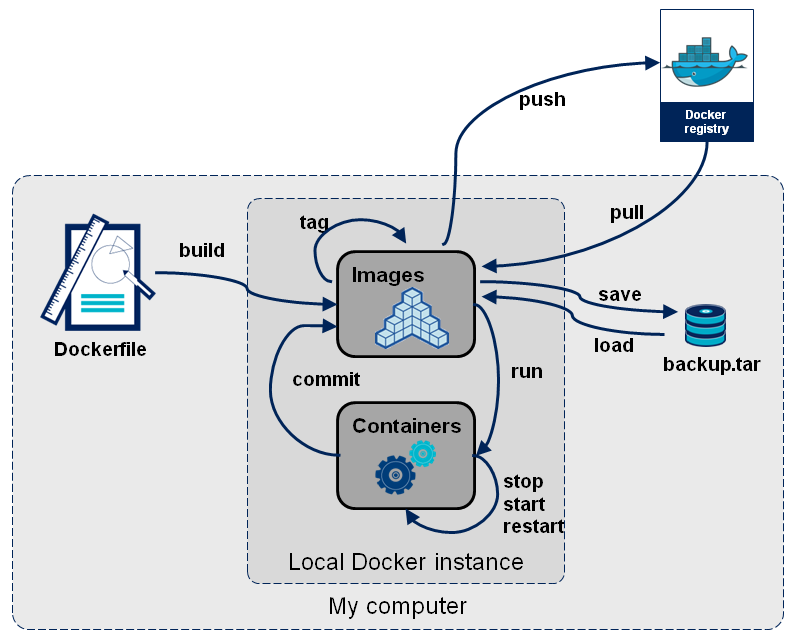
\includegraphics[width=0.7\linewidth]{imagens/docker-stages}
	\caption{Fluxo de disponibilização de Imagem Docker}
	Fonte: OCTO Technology\footnotemark	
	\label{fig:docker-stages}
	
	\footnotetext{Disponível em: https://blog.octo.com/en/docker-registry-first-steps/}
\end{figure}
\newpage
\subsection{Puppet}
É uma ferramenta de código livre para gestão de configurações. A ideia central do Puppet\footnote{Disponível em https://www.puppet.com/} é a administração de diversas máquinas físicas ou virtuais, onde a configuração é centralizada em um único nó e então distribuídas por diversos nós na rede, assim, gerenciando configurações, automatizando instalação de pacotes e facilitando o estabelecimento de normas e auditoria.\cite{walberg2008automate}

A ferramenta está disponível em duas versões: Puppet Enterprise\footnote{Disponível em: https://puppet.com/products/puppet-enterprise} (com suporte pago), e a Open Source Puppet\footnote{Disponível em: https://puppet.com/download-open-source-puppet} (código aberto). É uma ferramenta bem utilizada pela comunidade e por isso existem muitos módulos desenvolvidos, empresas como McAfee e Nasa fazem uso dela.

O Puppet utiliza o serviço SSH para a conexão aos hosts, esse é um ponto positivo se olharmos pela ótica que em alguns cenários não é possível a instalação de agentes ou em situações onde o agente consome uma fatia considerável de memória e cpu.\cite{puppet}

Na Tabela \ref{tab:tabelacomparativa1}, podemos fazer uma análise comparativa de funcionalidades e características, entre algumas ferramentas que concorrem na mesma categoria que o Puppet.

\begin{table}[h]
	\centering

	\begin{tabular}{|p{3.0cm}|p{3.0cm}|p{3.0cm}|p{3.0cm}|}
		\cline{1-4}
		
		  & Ansible &Puppet & Chef \\ % Note a separação de col. e a quebra de linhas
		\hline                               % para uma linha horizontal
		Linguagem do Script & YAML        & Custom DSL baseado em Ruby & Ruby\\ \cline{1-4}
		
		Infraestrutura & Máquina controladora aplica configuração em nós via SSH  & Puppet Master sincroniza configuração em nós Puppet & Chef Workstation empurra configuração para o servidor Chef onde os nós Chef serão atualizados  \\ \cline{1-4}
		
		Softwares especializados requeridos para nós & Não & Sim & Sim\\ \cline{1-4}
		
		Fornece ponto de controle centralizado & Não, qualquer computador pode ser controlado &  Sim, via  Puppet Master & Sim, via servidor Chef \\ \cline{1-4}
		
		Terminologia de Scripts & Playbook/Roles & Manifests/ Módulos & Receitas/ Cookbooks \\ \cline{1-4}
		
		Ordem de Execução das Tarefas & Sequencial & Não sequencial & Sequencial \\ \cline{1-4}         
		
	\end{tabular}
	\caption{Comparativo entre Ferramentas de Gerenciamento de Configurações}
	\label{tab:tabelacomparativa1}
	Fonte: Digital Ocean\footnotemark
\end{table}
	\footnotetext{Disponível em: https://www.digitalocean.com/}


\subsection{Ansible}

O Ansible\footnote{Disponível em https://www.ansible.com} foi criado em 2012, por Michael DeHann, basicamente essa ferramenta gerencia configurações e orquestra tarefas. Nesse sentido ele implementa módulos para nós sobre SSH. Os módulos são distribuídos nos nós temporariamente que realizam a comunicação com a máquina de controle (assim com em ferramentas concorrentes) por meio de um protocolo JSON\footnote{Disponível em: http://jsonapi.org/}.\cite{imhofsurvey}

O diferencial do Ansible em relação as demais ferramentas que se propõe ao mesmo objetivo, é que ele atua com uma arquitetura cliente-servidor, sem agente,  isso que dizer que os nós não são necessários para a instalação dos daemons para comunicação com a máquina controle. Isso resulta em diminuição de carga na rede. 

Os objetivos mais notáveis do Ansible é tornar a experiência do usuário muito mais simples e fácil, e investir massivamente na segurança e confiabilidade utilizando o \textit{OpenSSH} como condutor de dados. É uma linguagem construída tendo como parâmetro a auditabilidade, ou seja, possibilitar ao analista o acompanhamento de todas as etapas, rotinas e dados circulados dentro de uma arquitetura definida.\cite{marcelocosta}

Nessa ferramenta ainda encontramos o uso de um arquivo de inventário, denominado "hosts", que definem quais nós serão gerenciados, que é simplesmente um arquivo de texto que lista os nós individualmente ou agrupados, ou até um arquivo executável que constrói um inventário de hosts. É uma opção de alta confiabilidade e segurança, e isso se fundamenta pelo uso do \textit{Secure Shell}. Possui ainda fácil usabilidade, no entanto, não deixa a desejar em qualquer aspecto se comparado a soluções concorrentes.

Na forma tradicional de trabalho o Ansible faz o \textit{upload} do código que deve ser executado nas estações clientes, é então executado, retorna o resultado da execução e após isso é removido dos clientes. Quando usamos a ótica DevOps esse tipo de fluxo é modificado, fazendo uso do protocolo NETCONF\footnote{Disponível em: https://tools.ietf.org/html/rfc6241} (RFC 6241), onde é possível o envio de comandos aos componentes e receber o retorno da aplicação.

\subsubsection{Componentes}
O Ansible é estruturado pela composição dos seguintes elementos:

\begin{itemize}
	\item Playbooks\footnote{Disponível em https://docs.ansible.com/ansible/playbooks.html}: arquivos de configuração, implementação e linguagem de orquestração do Ansible.
	\item Agentless\footnote{Disponível em https://dbruno.ansible.com/ansible/}: É descartado o uso de agente nos servidores a serem monitorados. Isso deve-se à utilização de \textit{OpenSSH} para definir o estado atual do ambiente, adaptando-se se acaso estiver em desconformidade com a configuração no playbook.
	\item Módulos\footnote{Disponível em https://docs.ansible.com/ansible/modules.html}: São as tarefas executadas de fato. Os módulos são ditos como "plugins de tarefas" e por isso são eles que realizam as atividades pertinentes.
	\item Inventário\footnote{Disponível em https://dbruno.ansible.com/ansible/}: Armazena e controla informações sobre os grupos de hosts.
\end{itemize}

\subsubsection{Vantagens}
Podemos apontar alguns ganhos consideráveis na utilização do Ansible.
\begin{itemize}
	\item Não há a necessidade na instalação de agentes nos servidores a serem gerenciados;
	\item Gerencia paralela e simultaneamente de forma orquestrada; 
	\item Simples configuração e bem estruturado;
	\item Desenvolvimento em diversas linguagens.
\end{itemize}

\subsection{GitHub }
É um dos serviços web de repositórios mais difundidos. Com essa ferramenta é possível hospedar projetos e aplicações, trabalhando com controle de versionamento.

O Github\footnote{Disponível em https://www.github.com} funciona por meio de repositórios, que se dividem em pastas e dentro destas, subpastas que comportam os arquivos de diversas extensões e linguagens. Ainda oferece a possibilidade de contribuir com um código mesmo que não seja membro original do projeto, desde que permitido. Além de permitir o acesso múltiplo por diversos desenvolvedores de uma mesma empresa, permitindo que vários programadores trabalhem simultaneamente em uma mesma aplicação ou arquivo.\cite{bell2015introduccao}

Essa ferramenta funciona através de comandos "git", que gera ações de \textit{upload, request, clone, update, remove, merge e rollbacks} (retorno a versões anteriores do código). O git é estruturado em árvores, e nessa estrutura encontramos os \textit{Branchs} que são ponteiros que apontam para um determinado commit, como demonstra a Figura \ref{fig:git}

\begin{figure} [htb]
	\centering
	\includegraphics[width=0.85\linewidth]{git}
	\caption{Fluxo commit e request}
	Fonte: Cloud Turbine\footnotemark
	\label{fig:git}
\end{figure}
	\footnotetext{Disponível em: https://www.cloudturbine.com/using-github-and-git/}

\subsection{Jenkins}

Essa ferramenta multiplataforma funciona como um servidor destinado a integração contínua que automatiza a execução de tarefas, possui código aberto e permite ao usuário total liberdade em sua operação.

Basicamente o Jenkins\footnote{Disponível em https://www.jenkins.io} atua em um conceito de integração contínua, onde o objetivo é agilizar tarefas que tradicionalmente demandam um tempo de excecução mais prolongado como compilação do projeto e execução de testes automatizados. Cada interação é analisada por um \textit{build} automatizado a fim de detectar possíveis erros de integração, isso permite que testes sejam realizados reduzindo problemas de updates e tornando o software mais coeso.\cite{atalay}

O Jenkins pode ser integrado ao Git, SVN, CVS, Maven, entre outros. É importante ressaltar que um ponto forte do Jenkins é a difusão entre a comunidade. Ele ainda possui mais de 1000 plugins disponíveis e utilizado por várias empresas de desenvolvimento de softwares.\cite{ouverney2018automaccao}

Um recurso interessante é o uso de \textit{Forks} (recurso do GitHub), que permitem a criação de cópias de um determinado projeto e trabalha nesse sem a preocupação de afetar em algum ponto a aplicação original. É possivel ainda, adicionar testes de desempenho e balanceamento na integração contínua, permitindo a análise de risco e a reduzir eventuais quedas de performance no momento em que um novo recurso é adicionado ou a correção de um erro presente.\cite{ouverney2018automaccao}

\subsubsection{Vantagens}
As principais vantagens do Jenkins podem ser destacadas abaixo:
\begin{itemize}
\item \textit{Builds} periódicos;
\item Testes automatizados;
\item Possibilita análise de código;
\item Identificar erros mais cedo;
\item Fácil de operar e configurar;
\item Comunidade ativa;
\item Integra outras ferramentas por meio de plugins nativos.
\end{itemize}

\subsection{Sonar}

O SonarQube\footnote{Disponível em: https://www.sonarqube.org/} é uma plataforma de análise da qualidade do código, com ele é possível avaliar por meio de dados estatísticos o desempenho de determinada aplicação quanto aos testes realizados utilizando diversas métricas. 

A qualidade do código é verificada através de alguns eixos, como na Figura \ref{fig:7axessonar}, sendo esses, a arquitetura, duplicações de código, complexidade, regras de codificação, comentários, testes unitários e erros em potencial.

\begin{figure}[htb]
	\centering
	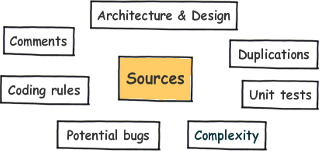
\includegraphics[width=0.5\linewidth]{imagens/7axes_sonar}
	\caption{7 Eixos de Análise do Sonar}
	Fonte: Blog Gabriel Amorim\footnotemark
	\label{fig:7axessonar}
\end{figure}
	\footnotetext{Disponível em: http://blog.gabrielamorim.com/analisando-a-qualidade-do-codigo-com-o-sonar/}

O Sonar tem compatibilidade com diversas linguagens, e plugins para vários serviços como Jenkins, por exemplo. Assim, é possível através da execução de uma determinada tarefa, definir métricas de análise, monitorar todo o processo e como retorno disponibilizar dados estatísticos referente a cada teste executado.\cite{cabralrelato}

Vantagens:
\begin{itemize}
	\item Fácil acompanhamento da evolução do código;
	\item Representação dos dados através de gráficos;
	\item Uso simples da ferramenta.
\end{itemize}

\subsection{Kubernetes}

O Kubernetes\footnote{Disponível em: https://kubernetes.io/} é um sistema destinado à orquestração de contêineres. É perfeitamente associável a ferramentas como Docker, Rocket, Jenkins, Chef, Puppet e Ansible. O seu objetivo é retirar o peso de execução de determinado contêiner em uma única instância do serviço, para isso o Kubernetes cria nós ou slaves diferentes e distribui a execução da tarefa entre esses nós. A figura \ref{fig:kubernetes} demonstra a arquitetura comum do Kubernetes.

\begin{figure}[htb]
	\centering
	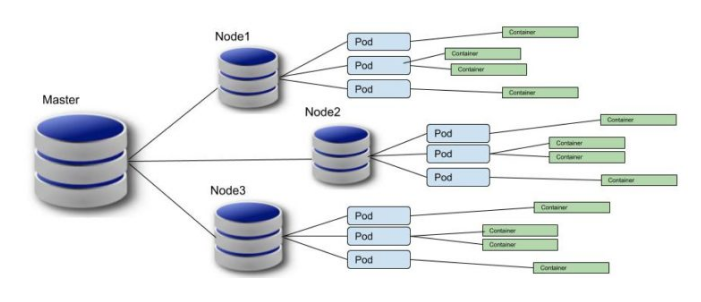
\includegraphics[width=1\linewidth]{imagens/kubernetes}
	\caption{Arquitetura do Kubernetes}
	Fonte: King Host\footnotemark
	\label{fig:kubernetes}
\end{figure}
	\footnotetext{Disponível em: https://king.host/blog/2018/05/introducao-ao-kubernetes/}

Instituições como \textit{Google} revelaram que utilizam  contêineres em serviços como \textit{Gmail} e \textit{Google Docs}, nesses são mais de 2 bilhões de implantações por semana, essa dinâmica é gerida pelo Borg, e essa mesma ferramenta foi precursora do Kubernetes. Em 2015 foi doada para a \textit{"Native Computing Foundation"} e \textit{"Linux Foundation"}, sendo a partir disso um projeto\textit{ open source}.\cite{trucco}
\newpage
Conforme a Figura \ref{fig:kubernetes}, a arquitetura do Kubernetes pode ser definida como:
\begin{itemize}
\item \textbf{Master:} é a instância central que provê uma determinada aplicação com configurações específicas.
\item \textbf{Cluster: }conjunto dos componentes. Na figura \ref{fig:kubernetes} percebemos a criação de um cluster.
\item \textbf{Node:} Uma máquina ativa gerenciada pelo master, pode também ser mencionada como \textit{minions} ou \textit{slaves}.
\item \textbf{Pods:} menores unidades implantadas que podem ser criadas, escaladas e manuseadas. É uma coleção lógica de contêineres que pertencem a uma aplicação.
\end{itemize}

O principal motivo que atrai desenvolvedores para o uso do Kubernetes é viabilizar aos \textit{clusters} abranger alocações em clouds públicas, privadas ou híbridas, e mais especificamente ainda, quando essa arquitetura envolve uma gama elevada de contêineres, o que exige que a ferramenta seja obrigatoriamente auto-escalável e proporcione alta disponibilidade.\cite{netto2016replicaccao}

\subsubsection{MiniKube}
O manuseio do Kubernetes é mais complexo do que seu concorrente direto \textit{Docker Swarm}\footnote{Disponível em: https://docs.docker.com/engine/swarm/}, demanda mais conhecimento de redes e sistemas distribuídos do arquiteto projetista do ambiente.

Pensando nisso a comunidade criou o Minikube\footnote{Disponível em: https://kubernetes.io/docs/setup/minikube/}, que basicamente é uma \textit{Toolkit} que reúne uma série de soluções que facilitam muito a implantação do Kubernetes, isso tornou a aplicabilidade mais abrangente, sendo possível o uso em plataformas Windows, Linux e Mac. Nesse caso, o Minikube simula um nó com tudo o que é preciso já instalado e configurado.\cite{mceniry2017kubernetes}


Vantagens:
\begin{itemize}
\item Fácil manipulação de contêineres;
\item Escalonamento da aplicação;
\item Volumes persistentes;
\item Auto regeneração;
\item Abstração de complexidade.
\end{itemize}

Desvantagens:
\begin{itemize}
\item Pouca documentação disponível para iniciantes;
\item Curva de aprendizado longa;

\end{itemize}



